\cotefile{156-8}
\scanpage{26}
\mspage{17}
% archive sheet number: 26

% source lines 1--4
3°) Mag 3 \textcircled{a} \textcircled{b} \unsure{trivial}, puisque $\unsure{|0|\,|\,|\circ|}$ n'a pas changé; et $\overset{\circ}{\ll}_{\unsure{\mathrm{pol}|\mathrm{pré}}}\ \Longrightarrow\ \deleted{\unsure{\ll}}\overset{\circ}{\ll}$.

4°) Mag 4 \deleted{aussi} n'a pas changé (ne fait intervenir que $\leq$ et $|0|$).

% source lines 5--12
\uline{Définition} Un magasin est dit \deleted{\unsure{pré}}\uline{polyédral}, si $X\ll Y\Longrightarrow X\ll_{\mathrm{pol}}Y$ (auquel cas il est \deleted{\unsure{un poly}} aussi prépolyédral, comme on voit en prenant $X\leq Y$), \deleted{Si $M,\leq,\ll,|0|$} donc si $\ll$ et $\ll_{\mathrm{pol}}$ sont égales dans $M$. Le magasin $M^{\mathrm{pol}}=(M,\leq,\ll_{\mathrm{pol}},|0|)$ est dit le magasin polyédral associé au magasin prépolyédral $M$\inserted{(il est bel et bien polyédral)}.

On a \deleted{\unsure{visiblement} $(M^{\mathrm{pol}})^{\mathrm{pol}}=M^{\mathrm{pol}}$, et} $M=M^{\mathrm{pol}}$ ssi $M$ est polyédral.

% source lines 13--16
\deleted{\unsure{Types de}} Mais même si $M$ est déjà polyédral, i.e. il n'y a pas à faire de différence entre $\ll$ et $\ll_{\mathrm{pol}}$, il \deleted{faut} distinguer deux notions de compatibilité, $\unsure{\gtrless|\lessgtr}$ et $\gtrless_{\mathrm{pol}}$.

% source lines 17--20
\uline{Définition} Soit $M$ magasin. On pose
\[
\begin{aligned}
 X\gtrless_{\mathrm{pol}}Y\ &\overset{\mathrm{def}}{\Longleftrightarrow}\ X\gtrless Y,\ \text{\uuline{et}}\ \forall X'\in\widetilde X,\ Y'\in\widetilde Y,\\
 &\widetilde{X'}\cap\widetilde{Y'}\text{ est vide ou a un}\\
 &\text{plus grand élément}
\end{aligned}
\]
% slanted
\margin{Il est clair que $X\gtrless_{\mathrm{pol}}Y$ et $X'\leq X$, $Y'\leq Y$ $\Longrightarrow X'\gtrless_{\mathrm{pol}}Y'$.}

% source lines 21--23
\uline{Donc} $M$ est prépolyédral ssi pour $\forall X\in M$, on a \deleted{$X$ et $Y,Z\leq X$, on a $Y\gtrless_{\mathrm{pol}}Z$. \unsure{Donc on a}} $X\gtrless_{\mathrm{pol}}X$, donc $Y\gtrless_{\mathrm{pol}}Z$ pour $Y,Z\leq X$.

% source lines 24--26
On introduit donc \deleted{\unsure{Fig}} $\mathrm{Fig}_{\mathrm{pol}}(M)\subset\mathrm{Fig}(M)$ (anciennement $\unsure{\mathcal F_M|F_M}$) formé des figures $F$ telles que $\forall X,Y\in\widetilde F$, on a $X\gtrless_{\mathrm{pol}}Y$,

\scanpage{27}
\mspage{18}
% archive sheet number: 27

% source lines 1--6
 i.e. des \deleted{figures} parties $F\subset M$ telles que
\[
\begin{aligned}
\text{a)}\quad &F\text{ fermé pour }\leq\\
\text{b)}\quad &X,Y\in F\ \Longrightarrow\ X\unsure{\gtrless|\lessgtr}_{\unsure{\mathrm{pol}|\mathrm{pré}}}Y,\quad\text{i.e.}\quad
\left\{\begin{aligned}
&\text{1°)}\ X'\in\deleted{\widetilde X}\widetilde X\cap\widetilde Y,\ Y'\in\deleted{\widetilde X}\widetilde X\cap\widetilde Y\\
&\hspace{2em}\Longrightarrow X'\unsure{|0|\,|\,|\circ|}Y'\\
&\text{2°)}\ \forall X'\in\widetilde X,\ Y'\in\widetilde Y,\ \widetilde X\cap\widetilde Y\\
&\text{est vide ou a un}\\
&\text{plus grand élément.}
\end{aligned}\right.
\end{aligned}
\]

\deleted{Ceci posé, on trouve}

% source lines 7--10
\uline{NB} Même si $M$ est polyédral, on aura en général une inclusion \uline{stricte} $\mathrm{Fig}_{\mathrm{pol}}(M)\subsetneq\mathrm{Fig}(M)$.

\figure{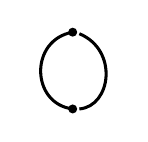
\begin{tikzpicture}[scale=.65]
\draw[line width=1.1pt] (0,.75) .. controls (-.85,.6) and (-.82,-.65) .. (0,-.75);
\draw[line width=1.1pt] (.13,.72) .. controls (.9,.4) and (.75,-.7) .. (.13,-.75);
\fill (0,.75) circle (2.5pt);\fill (0,-.75) circle (2.5pt);
\end{tikzpicture}}
Cette figure circulaire est dans $\mathrm{Fig}(M)$, mais non dans $\mathrm{Fig}_{\mathrm{pol}}(M)$, pour $M$ magasin polyédral \unsure{convenable}.

% left margin, with two drawings
\margin{Exemple analogue avec $X\ll Y$ mais non $X\ll_{\mathrm{pol}}Y$ (\unsure{à l'intérieur des} \unsure{2-simplexes|2-simples})}
\figure{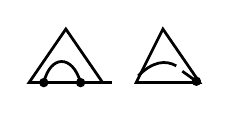
\begin{tikzpicture}[scale=.85]
\draw[line width=1pt] (0,0)--(.55,.8)--(1.1,0)--cycle;
\draw[line width=1pt] (.22,0) .. controls (.32,.42) and (.65,.42) .. (.77,0);
\fill (.22,0) circle (2pt);\draw[line width=1pt] (1.1,0)--(1.24,0);\fill (.77,0) circle (2pt);
\draw[line width=1pt] (1.6,0)--(2,.8)--(2.55,0)--cycle;
\draw[line width=1pt] (1.63,.1) .. controls (1.85,.32) and (2.04,.34) .. (2.2,.25);
\draw[line width=1pt] (2.29,.17)--(2.5,.02);
\fill (2.5,.02) circle (2pt);
\end{tikzpicture}}

% source lines 11--18
\uline{Scholie} Les propriétés \inserted{algébriques} formelles de $\unsure{\mathcal F|F}=\mathrm{Fig}_{\mathrm{pol}}(M)$, muni des $\leq,\ll_{\mathrm{pol}},\gtrless_{\mathrm{pol}}$, et ses relations avec $M$ (muni des relations induites) seront sensiblement les mêmes que pour $\leq,\ll_{\deleted{\mathrm{pol}}},\gtrless_{\deleted{\mathrm{pol}}}$. \deleted{\unsure{et}} La seule différence est dans l'explicitation de $\gtrless_{\mathrm{pol}}$ \unsure{resp.} $\gtrless$, en termes de la relation de disjonction interne $|0|$.

On devrait passer en revue \deleted{toutes} les propositions pertinentes\ldots

Je signale seulement celle-ci

% source lines 19--24
\uline{Prop} Si $F,G\in\mathrm{Fig}_{\mathrm{pol}}$, alors \deleted{$\{F,G\}$ \unsure{majoré}} conditions équivalentes
\[
\begin{aligned}
\text{(i)}\quad &\{F,G\}\text{ majoré pour }\leq\\
\text{(ii)}\quad &\mathrm{Sup}^{\leq}(F,G)\text{ existe}\\
\text{(iii)}\quad &F\cup G\text{ (réunion dans }\unsure{\mathcal P|\mathscr P}(M)\text{)}\in\mathrm{Fig}_{\mathrm{pol}}(M)\\
\text{(iv)}\quad &\forall X\in\widetilde F,\ Y\in\widetilde G,\text{ on a }X\gtrless_{\mathrm{pol}}Y.
\end{aligned}
\]
\margin{On écrit alors $F\gtrless_{\mathrm{pol}}G$}

% source lines 25--29
Dans certains contextes, on laissera tomber l'indice pol à $\gtrless$, $\ll$, quand il est bien entendu qu'il ne s'agit que des relations ``polyédrales''.

\uline{Atelier polyédral} Se définit essentiellement \inserted{(en termes d'un \unsure{magasin} polyédral $M$ et de $\mathrm{Fig}_{\mathrm{pol}}(M)$,)}

\scanpage{28}
\mspage{19}
% archive sheet number: 28

% source lines 1--7
 de la même façon qu'un atelier ``spacieux'' (ou ordinaire) se définit en termes d'un magasin quelc. et de $\mathrm{Fig}(M)$. En termes d'un $\unsure{\mathcal F|F}\subset\unsure{\mathcal P|\mathscr P}(M)$, ou plutôt $\mathcal F\subset\mathrm{Fig}_{\unsure{\mathrm{pol}|\mathrm{pré}}}(M)$, les axiomes pertinents, qui \unsure{paraphrasent} Mag at (p.~10) est

% source lines 8--12
\uline{Mag at pol}
\[
\begin{aligned}
\text{a)}\quad &F\in\mathcal F,\ G\leq F\text{ (i.e. }G\text{ partie fermée de}\\
&F\text{ pour }\leq\text{ dans }M)\ \Longrightarrow G\in\mathcal F\\
\text{b)}\quad &F,G\in\mathcal F,\ F\unsure{\gtrless|\lessgtr}_{\mathrm{pol}}G\ \Longrightarrow F\cup G\in\mathcal F\\
\text{c)}\quad &\forall \unsure{x|X}\in M,\ \widetilde x\in\mathcal F\\
\text{c')}\quad &\mathcal F\neq\varnothing\quad(\Longleftrightarrow\varnothing\in\mathcal F).
\end{aligned}
\]

% source lines 13--22
\uline{NB} Un ``atelier spacieux'' \uline{est} \inserted{aussi} un ``atelier polyédral'' ssi le magasin associé est polyédral, \deleted{et si} \deleted{si de plus} (i.e. $X\ll Y\Longrightarrow X\ll_{\mathrm{pol}}Y$) \deleted{et si} (chose qui n'est pas vraie), et si \uline{de plus}, $X\gtrless Y\Longrightarrow X\gtrless_{\mathrm{pol}}Y$ (ce qui est beaucoup plus exceptionnel(?)). Il vaut mieux se faire une raison que ce sont des notions très voisines, mais \unsure{disparates}, et que
% slanted
\margin{Cela provient \unsure{seulement} du point de vue \unsure{choisi}, où on a pris $\ll$ comme relation primitive, mais non $\gtrless$. Il y a là un certain arbitraire\ldots}

% source lines 23--26
 a) Les notions ``spacieuses'' \deleted{\unsure{les}} $\ll$, $\gtrless$ sont plus commodes quand il s'agit de travailler avec des figures aussi générales que possibles, et que

% source lines 27--33
 b) Les notions ``polyédrales'' $\ll_{\mathrm{pol}}$, $\gtrless_{\mathrm{pol}}$ sont plus commodes quand il s'agit de travailler avec des figures, \unsure{vues|vus} comme des ``découpages'' \inserted{\unsure{d'autres|d'icelles}} en ``morceaux'' aussi ``standard'' que possible, avec des ``\unsure{ajustement|ajustements} \deleted{\unsure{standard}} des morceaux'' aussi \deleted{\unsure{S|A}} standard que possible.

\scanpage{29}
\mspage{20}
% archive sheet number: 29

% source lines 1--7
Dans le magasin, la différence des deux points de vue se réduit au minimum. On ne la voit pas dans la nature des données, \deleted{et des axiomes} à cela près que dans le cas ``polyédral'', on demande des axiomes plus stricts, savoir, en plus de Mag 1--Mag 4, l'\uline{axiome supplémentaire}

% source lines 8--10
\uline{Mag pol} Pour $X\ll Y$ et $Y'\in\widetilde Y$, $\widetilde X\cap\mathrm{Omb}(Y')$ est vide, ou a un plus grand élément, qui exprime que $X\ll Y\Longrightarrow X\ll_{\unsure{\mathrm{pol}|\mathrm{pré}}}Y$.

% source lines 11--13
Cela n'empêche qu'il faudra par la suite, en plus de $\unsure{\gtrless|\lessgtr}$, (ou \uline{au lieu} de $\gtrless$), introduire la relation $\gtrless_{\mathrm{pol}}$\unsure{\ldots|.}

% isolated oblique separator stroke
\figure{\begin{tikzpicture}\draw (0,1.6)--(1.1,0);\end{tikzpicture}}

% source lines 14--18
Je reviens encore sur l'axiomatique de base en termes de Mag 1 : Mag 4, en notant que la connaissance de $\overset{\circ}{\ll}$, $\unsure{|0|\,|\,|\circ|}$ redonne celle de $\ll$ par l'équivalence
\[
X\ll Y\Longleftrightarrow\exists Y',\quad X\overset{\circ}{\ll}Y'\leq Y.\tag*{($\ast$)}
\]

% source lines 19--23
On se demande, dès lors, quand \deleted{\unsure{M}} \inserted{\unsure{on part}} \deleted{\unsure{étant donné}} \inserted{d'une donnée}
\[
(M,\overbrace{\leq,\overset{\circ}{\ll}}^{\inserted{\text{rel. d'ordre}}},|0|),
\]
\deleted{quand} celle-ci provient d'un magasin. Il faut donc examiner les conditions pour que

\scanpage{30}
\mspage{21}
% archive sheet number: 30

% source lines 1--4
 a) $(M,\leq,\ll,\unsure{|0|\,|\,|\circ|})$, où $\ll$ défini par $(\ast)$, est un magasin, et

 b) La relation de raffinement immédiat dans ce magasin est la relation de départ $\overset{\circ}{\ll}$.

% source lines 5--10
Il faut supposer déjà
\[
\inserted{\leq,}\ \overset{\circ}{\ll}\quad\deleted{\text{est une}}\ \inserted{\text{sont des}}\ \text{relations d'ordre},\tag*{\textcircled{A}}
\]
et pour vérifier Mag 1, il reste à vérifier que $X\ll Y$ est une relation d'ordre. Ceci se ramène à la situation (qu'il faut \unsure{sans doute poser en axiome})
\[
X\leq Y\overset{\circ}{\ll}Z\ \Longrightarrow\ \deleted{\unsure{\forall}}\exists\deleted{\unsure{\forall|!}}\,Z'\text{ avec }X\overset{\circ}{\ll}Z'\leq Z,\tag*{\textcircled{B}}
\]
avec même l'\uline{unicité} de $Z'$. \deleted{\unsure{Dans le premier cas}} \unsure{unicité à part comme}

% source lines 11--13
\deleted{\uline{Mag 2}}
\margin{\uline{avant B}}
\textcircled{B'} Si $X$ \unsure{\&|et} $Y$ tels qu'il existe $Y'$ avec $X\overset{\circ}{\ll}Y'\leq Y$, alors $Y'$ est unique.

% source lines 14--18
Dans ces conditions, Mag 2 devient automatique ainsi que le fait que si $X\overset{\circ}{\ll}Y$, alors \deleted{$Y$ \unsure{est}} \deleted{\unsure{élément}} $X\ll Y'\leq Y\Longrightarrow Y'=Y$ (i.e. $X$ est raffinement immédiat de $Y$, au sens des \unsure{op. rel.} $\leq$, $\ll$).

\uline{Mag 3} reste ne varietur, en \textcircled{\unsure{3|B}}. Mag 4 aussi.

% source lines 19--27
En résumé, l'axiomatique devient
% slanted
\margin{\unsure{Axiomes}}

\uline{Mag 1'} $X\leq Y$ et $X\overset{\circ}{\ll}Y$ sont des relations d'ordre.

\uline{Mag 2'} a) Soient $X,Y$ tels qu'il existe $Y'$, avec $X\overset{\circ}{\ll}Y'\leq Y$. Alors cet $Y'$ est uniquement déterminé.
% slanted
\margin{relations entre $\leq$ et $\overset{\circ}{\ll}$}

 b) Si $\deleted{\unsure{\overset{\circ}{\ll}}}X\overset{\circ}{\ll}Y$, alors $\forall X'\unsure{\in|\leq}\widetilde X$, \inserted{il existe} $Y'\in\widetilde Y$ avec $X\overset{\circ}{\ll}Y$ (NB $Y'$ unique par a)).

\uline{Mag 3'}, \uline{Mag 4'} comme \uline{Mag 3}, \uline{Mag 4}
% slanted
\margin{\uline{Mag 3'} relation entre $\overset{\circ}{\ll}$ et $|0|$}
% slanted
\margin{\uline{Mag 4'} relation entre $\leq$ et $|0|$}

% source lines 28--29
Ce n'est pas plus simple ni moins simple que Mag 1--Mag 4, mais la donnée de $\overset{\circ}{\ll}$ paraît

\scanpage{31}
\mspage{22}
% archive sheet number: 31

% source lines 1--8
plus ``primaire'' que celle de $\leq$ \inserted{et plus ``naturelle''}, car

1°) Elle est ``disjointe'' de \deleted{\unsure{elle}} donnée $\leq$, en fait on a $(X\leq Y\text{ et }X\overset{\circ}{\ll}Y)\Longleftrightarrow X=Y$, \deleted{et}

et 2°) elle intervient plus naturellement dans Mag 3 = Mag 3'. On peut dire \deleted{\unsure{aussi}} \inserted{ainsi} que les axiomes \deleted{MAG} Mag 1'--Mag 4' sont à fonctions plus clairement séparées. Je vais les reformuler légèrement.

% source lines 9--11
\uline{Mag 1'} \inserted{(Nature interne des trois relations séparément)} $X\leq Y$ et $X\overset{\circ}{\ll}Y$ sont des relations d'ordre. $X\deleted{\unsure{\nparallel|\nmid}}\unsure{|0|\,|\,|\circ|}Y$ est une relation symétrique\unsure{,|.} \unsure{antiréflexive|anti-réflexive}.
% slanted
\margin{distinguer a) b) c)}
% slanted
\margin{Dans la version finale, ce seront ces axiomes \unsure{bien sûr qui} s'appelleront \uline{Mag 1 : Mag 4}}

% source lines 12--15
\uline{Mag 2'} (Relations entre $\leq$ et $\overset{\circ}{\ll}$)

 a) Si $X\overset{\circ}{\ll}Y'\leq Y$, $Y'$ est unique en termes de $X,Y$

 b) Si $X\overset{\circ}{\ll}Y$, alors $\forall X'\in\widetilde X,\ \exists Y'\in\widetilde Y$ tel que $X'\overset{\circ}{\ll}Y'$.

% source lines 16--17
\uline{Mag 3'} (Relations entre $\overset{\circ}{\ll}$ et $|0|$)

Si $X|0|Y$, $X'\overset{\circ}{\ll}X$, $Y'\overset{\circ}{\ll}Y$, alors $X'|0|Y'$

% source lines 18--19
\uline{Mag 4'} (Relations entre $|0|$ et $\leq$) Si $X\leq Y$, $X\neq Y$, alors $\unsure{\neg}\ X|0|Y$.

% source lines 20--21
Décidément, c'est la forme parfaite de définition !

% source lines 22--24
Rappel du périple parcouru depuis \deleted{trois}\inserted{plus} semaines, pour le choix des données de base, depuis \unsure{CF|GF} IV p.~52 (\deleted{\unsure{jeu}} 13 juin)

% source lines 25--29; aligned historical list
\diagram{\begin{tabular}{@{}l p{.62\linewidth}@{}}
$\deleted{\unsure{M,\ll,\leq|M,\leq,\ll}}\unsure{\mathcal F|F},\leq,\unsure{\preccurlyeq|\preceq}$ & \\
$\mathcal F,\leq,\ll$ & \\
$M,\leq,\ll,\unsure{\gtrless|\lessgtr}$ & (retour vers les origines) \inserted{ou $M,\leq,\ll,\parallel$ (grand \unsure{scandale})} \\
$M,\leq,\ll,|0|$ & innovation d'avant-hier faisant tomber tout le \unsure{fouillis} des axiomes de compatibilité-disjonction \\
$M,\leq,\overset{\circ}{\ll},|0|$ & aujourd'hui, l'\unsure{épurement} intégral !
\end{tabular}}

\scanpage{32}
\mspage{23}
% archive sheet number: 32

% source lines 1--7
Ce choix d'\deleted{axiomes} données de base
\[
\leq,\quad\overset{\circ}{\ll},\quad\unsure{|0|\,|\,|\circ|}
\]
force la main, pour ainsi dire, pour le choix correspondant pour \deleted{$\unsure{F}$} un atelier $\unsure{\mathcal F|F}$. Seule des trois relations primitives, $\leq$ passe à $\mathcal F$. Donc partir de $\mathcal F$ tout seul dès lors paraît \unsure{artificiel}, il vaut mieux prendre \deleted{$(M,\mathcal F$}
\[
(M,\mathcal F\unsure{;|\}}\ \triangleleft,\overset{\circ}{\ll},|0|)
\]
i.e. $\triangleleft$ ``relation d'incidence'' entre $M$ et $\mathcal F$ et $\overset{\circ}{\ll},|0|$ relations dans $M$ (les relations $\leq$, dans $M$ ou dans $\mathcal F$, ``sortent'' de $\deleted{\unsure{\leq}}\triangleleft$).

% source lines 8--15
Voyons la forme que prennent les \inserted{données} axiomes pour un ``magasin strictement divisible''$^\ast$ (cf p.~7). La relation $|0|$ est ici redondante, \deleted{D'abord} sur $M$, on se la donne (sous notation $\parallel$) sur $\uline{\unsure{L|\mathcal L}}$. D'autre part, en termes de $\deleted{\unsure{\forall}}\leq,\overset{\circ}{\ll}$, on définit $L$ comme
\[
L=\{X\in M\mid X\text{ minimal pour }\leq\text{ et pour }\overset{\circ}{\ll}\}.
\]
% slanted
\margin{$^\ast$ \unsure{ou} \unsure{Magasins où l'ens.|Magasins ou l'ens.} \unsure{lieux} (\uline{très \unsure{denses|dense}})}

% source lines 16--17
Donc données
\[
(M,\leq,\overset{\circ}{\ll},\parallel)\qquad\text{avec}
\]
% slanted
\margin{On retrouve $X|0|Y$ par $X|0|Y\Longleftrightarrow\forall x\overset{\circ}{\ll}X,\ y\overset{\circ}{\ll}Y$, on a $x\parallel y$.}

% source lines 18--22
\uline{Mag div 1} $\leq,\overset{\circ}{\ll}$ sont des relations d'ordre sur $M$. La relation $\parallel$ est une relation sym. et antiréflexive sur l'ens. $L$ des éléments de $M$ minimaux pour $\leq$ et $\overset{\circ}{\ll}$.

\uline{Mag div 2} Comme Mag \unsure{2'|1'} page précédente.

\uline{Mag div 3} Si $X\leq Y$, $X\neq Y$, $x\overset{\circ}{\ll}X$, $y\overset{\circ}{\ll}Y$, $x,y\in L$, alors $x\parallel y$. \deleted{\unsure{C'est le Mag}}

\scanpage{33}
\deleted{\unsure{26|21}}\mspage{\unsure{24|26}}
% archive sheet number: 33

Cas quasi-ensembliste où la relation $x\parallel y$ équivaut à $x\ne y$.

Données $(M,\leq,\overset{\circ}{\ll})$, avec axiomes

\uline{Mag quens 1}\quad $\leq$ et $\overset{\circ}{\ll}$ sont des relations d'ordre.

\uline{Mag quens 2}\quad Comme Mag $2'$ p. 21

\uline{Mag quens 3}\quad $\forall X\in M$, $\exists x\in\unsure{L|\mathcal L}$, avec $x\overset{\circ}{\ll}M$.

% slanted
\margin{On retrouve $X\unsure{|0|\,|\,|\circ|}Y$ par $X|0|Y\Longleftrightarrow\mathrm{omb}^{\unsure{\circ|0}}(X)\cap\mathrm{omb}^{\circ}(Y)=\varnothing$, où $\mathrm{omb}^{\circ}(Z)=\{x\in L\mid x\overset{\circ}{\ll}Z\}$.}

Enfin, les magasins ensemblistes (les seuls à vrai dire avec lesquels les gens \unsure{aient|ont} travaillé avant moi!) sont réduits à la structure de la p. 9, à laquelle \unsure{je n'ai|j'ai} rien à ajouter, sinon pour expliciter les structures $\leq$, $\ll$ comme induites par les structures ensemblistes correspondantes de $\operatorname{Fig}(L)$, et la \deleted{\unsure{loi}} relation
\[
X|0|Y\Longleftrightarrow X^\circ\cap Y^\circ=\varnothing
\]
où $X^\circ=X\setminus\unsure{\delta|\partial}X$, $Y^\circ=Y-\delta Y$, constructions ensemblistes habituelles.

\diagram{\scriptsize
\begin{tikzcd}[ampersand replacement=\&,column sep=small,row sep=small]
\overset{\text{(p. 22)}}{\text{Mag }1\text{--}4}\quad
\overset{\text{(p. 6,7)}}{\text{Mag L}1,\text{L}2},
\arrow[ddddr,no head,out=-20,in=100]\&
\overset{\text{(p. 10)}}{\text{Mag at}}\&
\text{pour des ``Magasins''}
\\
\deleted{\text{Mag At }1\text{--}5}\&\&
\\
\overset{\text{(p. 11,12)}}{\text{At }1\text{ -- At }5}\quad+\text{Mag }1\text{--}4\&\rule{2cm}{0.4pt}\&\text{ateliers}
\\
\overset{\text{(p. 13,14)}}{\text{At M}1\text{ -- At M}5}\quad+\text{Mag }1\text{--}4\&\rule{2cm}{0.4pt}\&\text{mixtes}
\\
\overset{\text{(p. 23)}}{\text{\uline{Mag div 1--3}}}\&\text{(au lieu de Mag }1\text{--}4,+\text{L}2\text{)}\&\rule{1cm}{0.4pt}\quad\text{magasins}
\\
\text{Mag quens }1\text{--}3\quad\text{(p. 24)}\&\&\rule{3cm}{0.4pt}
\\
\text{Mag ens }1\text{--}2\quad\text{(p. 9)}\&\&\rule{3cm}{0.4pt}
\end{tikzcd}
}

\diagram{\scriptsize
\begin{tikzcd}[ampersand replacement=\&,column sep=small,row sep=tiny]
\circ\arrow[r]\&\text{Variantes polyédrales}\quad\text{\uline{$\text{Mag }1\text{--}4+\text{Mag pol }(+\text{Mag At pol})$}}
\\
\&\text{(pages 15--19)}
\end{tikzcd}
}

\margin{! Voir aussi Mag $1'$, Mag $2'$ p. \unsure{38|30|28},\unsure{33|31}}
